
\mysubsection{Trajectoires}

\paragraph{Linéaire}
Pour faire la trajectoire linéaire, on a utilisé le polynôme de cinquième dégrée montré en \cite{khalil2004modeling}, $ 10(\frac{t}{t_f})^3-15(\frac{t}{t_f})^4+6(\frac{t}{t_f})^5 $, et modifié pour utiliser les entrées, de point initial, point final et le temps total du mouvement.

Par exemple, si le point initial $ p_i $, le point final $ p_f $ et le temps $ t_f $ sont connus, donc la position suive la fonction suivante:

\begin{equation}
	P(t)=(p_f-p_i)(10(\frac{t}{t_f})^3-15(\frac{t}{t_f})^4+6(\frac{t}{t_f})^5)+p_i
\end{equation} 

Pour un point initial $ p_i=[10,5,9] $, un point final $ p_f=[7,9,8] $ et temps final $ t_f=10s $

\begin{subequations}
	\begin{equation}
		X(t)=(7-10)(10(\frac{t}{10})^3-15(\frac{t}{10})^4+6(\frac{t}{10})^5)+10
	\end{equation}
	\begin{equation}
		Y(t)=(9-5)(10(\frac{t}{10})^3-15(\frac{t}{10})^4+6(\frac{t}{10})^5)+5
	\end{equation}
	\begin{equation}
		Z(t)=(8-9)(10(\frac{t}{10})^3-15(\frac{t}{10})^4+6(\frac{t}{10})^5)+9
	\end{equation}
\end{subequations}
\newpage
\begin{figure}[H]
	\centering
	\begin{minipage}[b]{0.45\textwidth}
		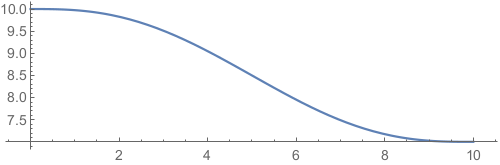
\includegraphics[width=\textwidth]{./parametrizacao_x}
		\caption{Graphique de la paramétrisation de X.}
	\end{minipage}
	\hfill
	\begin{minipage}[b]{0.45\textwidth}
		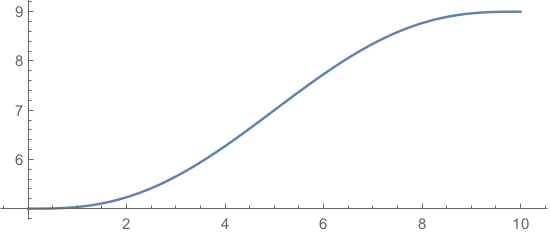
\includegraphics[width=\textwidth]{./parametrizacao_y}
		\caption{Graphique de la paramétrisation de Y.}
	\end{minipage}
\end{figure}


\begin{figure}[H]
	\begin{center}	
		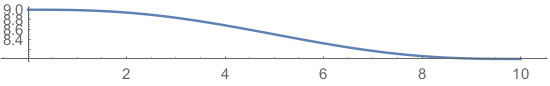
\includegraphics[width=8cm]{./parametrizacao_z}
		\caption{Graphique de la paramétrisation de Z.}
		\label{fig:parametrizacao_z}
	\end{center}
\end{figure}


\begin{figure}[H]
	\begin{center}	
		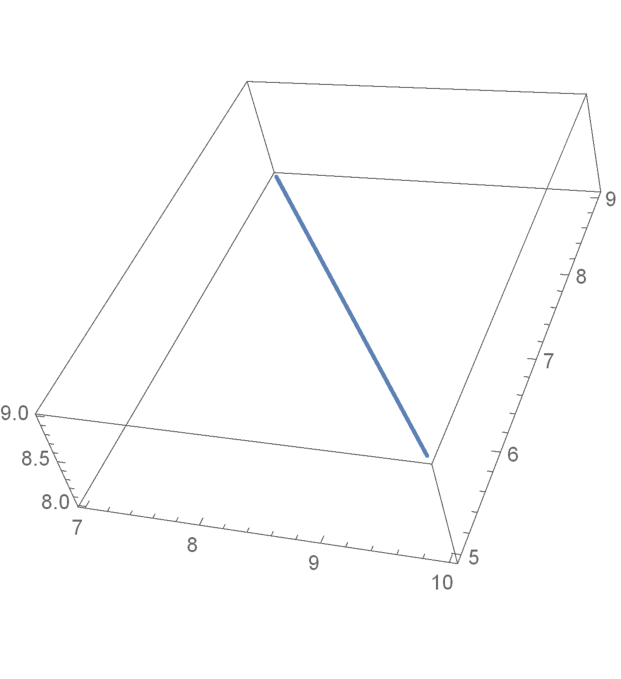
\includegraphics[width=8cm]{./trajectoire_1}
		\caption{Représentation tridimensionnel de la trajectoire}
		\label{fig:trajectoire}
	\end{center}
\end{figure}

\paragraph{Arc de cercle}

Dans un première moment on a choisi essayer de résoudre le problème  en deux dimensions.

Comme paramétrisation du cercle on a pensé en utiliser tel:

\begin{subequations}
	\begin{equation}
	X=1-cos(t)
	\end{equation}
	\begin{equation}
	Y=sin(t)
	\end{equation}
\end{subequations} 

Modifiant la fonction pour la généraliser et en faisant t varier de 0 a la valeur du angle entre les points initial et final et le centre du cercle.

On sait que les dérivatives (1ère et 2ème) de ces équations sont lisse mais ne sont pas prés de 0 au but e a la fin du mouvement, donc il faut aussi créer des polynômes interpolateurs, mais au même temps, attenter pour que la courbe résultante soit le plus prés possible d'un cercle.     